\documentclass[10pt, a4paper]{article}

\usepackage[utf8]{inputenc}
\usepackage{amsmath, amssymb, amsthm, bbm}
\usepackage{xcolor}
\usepackage{graphicx}
\usepackage[authoryear]{natbib}
\usepackage{apalike}
\usepackage{relsize}
\usepackage{array}
\usepackage{multirow}
\usepackage{showlabels}
\usepackage{setspace}
\usepackage[normalem]{ulem}
\usepackage{xspace}
%Add line numbering
%Line numbering can be incorporated by using the lineno package. Add these statements in the preamble:
\usepackage{lineno}
\linenumbers

\usepackage[nomarkers,figuresonly]{endfloat}

\DeclareMathOperator*{\argmax}{arg\,max}

\newtheorem{prob}{Problem}
\newtheorem{prop}{Proposition}
\newtheorem{definition}{Definition}

%%%%% bold symbol in math enviornment
\newcommand{\m}[1]{\boldsymbol{#1}}

\newcommand{\fmm}{\textsc{fmm}\xspace}

\newcommand{\pkg}[1]{{\fontseries{b}\selectfont #1}} 

\title{Merging the components of a finite mixture using  posterior probabilities}
\author{M. Comas-Cufí \and J.A. Martín-Fernández \and G. Mateu-Figueras}

%\doublespacing
\begin{document}

\begin{spacing}{1.9}
%%%%%%% BEGIN SPACING


\pagenumbering{arabic}

\maketitle

\section{Introduction}


% Mixture models
A common approach in parametric cluster analysis assumes data can be modelled by means of a \emph{finite mixture of distributions} \citep{fraley2002model}, also called \emph{finite mixture model} (\fmm). A \fmm is a probability distribution whose probability density function (pdf) is a linear combination of different distributions with same domain $\mathbb{X}$. More precisely, the pdf $f$ of a \fmm is
\begin{equation}\label{mixt}
f(\;\cdot\; ; \pi_1, \dots, \pi_k, \m\theta_1, \dots, \m\theta_k) = \pi_1 f_1(\;\cdot\; ; \m\theta_1) + \dots + \pi_k f_k(\;\cdot\; ; \m\theta_k),
\end{equation}
where $\m\theta_j$ is the set of parameters of the pdf $f_j$, $1\leq j \leq k$ and$\pi_j$ is the ``weight'' of component $f_j$. Note that taking $\sum_{\ell = 1}^k \pi_\ell = 1$ guarantees that  $\int_{\mathbb{X}}f = 1$. Originally, the clustering algorithm based on a \fmm follows two steps:
\begin{enumerate}
\item using the information provided by a sample $X= \{x_1, \dots, x_n\}$, to calculate estimates $\hat{\pi}_1, \dots, \hat{\pi}_k,$ $\hat{\m\theta}_1, \dots, \hat{\m\theta}_k$ of parameters $\pi_1, \dots, \pi_k,$ $\m\theta_1, \dots, \m\theta_k$, and
\item to classify each observation $x_i \in X$ according to the criterium of mazimizing the posterior probability, that is, one observation $\m x_i \in \mathbb{X}$ is classified to cluster $c$ if
\begin{equation}\label{map_criteria}
c=\argmax_{j=1}^k \frac{ \hat{\pi}_j f_j(\m x_i ; \hat{\m\theta}_j) }{\sum_{\ell=1}^k \hat{\pi}_\ell f_\ell(\m x_i ; \hat{\m\theta}_\ell) }.
\end{equation}
\end{enumerate}
Note that in this process, the number of clusters $k$ is equal to the number of mixture components. The decision concerning the value of $k$ is analyzed using different [citar referències].

More recently, \cite{lee2004combining,hennig2010methods,baudry2010combining,melnykov2013distribution,pastore2013merging} proposed to separate the concepts of cluster and component. The authors show that associating each mixture component to one cluster can be misleading because frequently two different mixture components are so overlapped that they can be considered as a unique cluster. In other words, one cluster could be formed by the result of merging two different mixture components. According to this approach, the clustering algorithm is completed with a third step:

\begin{itemize}
\item[3.] to analyse which of the $k$ clusters should be merged to form $k'$ clusters, $k' \leq k$.
\end{itemize}

The crucial point of this clustering method is how to decide which components have to be merged.


In this article we introduce a generic approach that contains the methods given by \cite{baudry2010combining}, \cite{hennig2010methods} and \cite{longford2014}. In addition, our approach permits to define its own criteria. As illustration we introduce a criteria based in log-ratio transformations \citep{aitchison1986statistical}. Using this approach for merging components one can build a hierarchy over the set of mixture components. From this hierarchical structure, the analyst can decide the final classification.

The paper is organised as follows: in Section~\ref{definitions} some definitions and notations used throughout this paper are introduced and specified using a simple example. In Section~\ref{generic_merging} the generic merging approach is presented. In Section~\ref{function_examples} is shown how different examples from literature reduce to the generic approach presented in the previous section. Section~\ref{logratio_section} presents a new family ofcriteria based on log-ratio approach. Finally, in Section~\ref{merging_examples_dist}, we present two examples to illustrate the algorithm with different types of mixture distributions.

\section{Definitions and notation}\label{definitions}

%
A \emph{partition} of $\{1, \dots, k\}$ of size $s$, $\mathcal{P}_s$,  is a set with $s$ subsets $I_p$ called $parts$ that $\bigcup_{I_p \in \mathcal{P}_s} I_p = \{1, \dots, k\}$ and for any two parts $I_a, I_b \in \mathcal{P}_s$ with $a \neq b$, $I_a \cap I_b = \emptyset$ holds. Note that for any partition  $\mathcal{P}_s$ the pdf $f$ of a \fmm (Equation~\ref{mixt}) can be rewritten as
\begin{equation}
f = \pi_{I_1} f_{I_1} + \dots + \pi_{I_s} f_{I_s},
\label{mixt_part}
\end{equation}
where $f_{I_p} = \sum_{j \in I_p} \frac{\pi_j}{\pi_{I_p}} f_j(\;\cdot\; ; \m\theta_j)$ and $\pi_{I_p} = \sum_{\ell \in I_p} \pi_\ell$. Moreover, note that using this notation each $f_{I_p}$ is also a \fmm.



A \emph{hierarchical sequence of partitions of $\{1,...,k\}$}, is a sequence $\mathcal{P}_1, \dots, \mathcal{P}_k$ verifying that
\begin{itemize}
\item $\mathcal{P}_1$ is the one-part partition $\mathcal{P}_1 = \{ \{1, \dots, k\} \}$,
\item for each $s$, $1 \leq  s \leq k$, $\mathcal{P}_{s}$ has $s$ subsets,
\item if a part $I_p \in \mathcal{P}_{s-1}$ then either there is a part $I_a \in \mathcal{P}_{s}$ with $I_p = I_a$ or there are two parts $I_a, I_b \in \mathcal{P}_s$ with $I_p = I_a \cup I_b$, and
\item $\mathcal{P}_k= \{ \{1\},\{2\}, \dots, \{k\} \}$.
\end{itemize}



One can extend Equation~\ref{map_criteria} in terms of partitions. Indeed, let $\rm X = \{\m x_1,\dots, \m x_n\}$ be a sample formed by observations of $\mathbb{X}$. Given a partition $\mathcal{P}_s = \{ I_1, \dots, I_s \}$ the posterior probability of $\m x_i$ being classified to part $I_p\in \mathcal{P}_{s}$ is
\[
\tau_{i I_p} =  \frac{ \hat{\pi}_{I_p} f_{I_p}(\m x_i; \hat{\theta}) }{\sum_{\ell=1}^s \hat{\pi}_{I_\ell} f_{I_\ell}(\m x_i; \hat{\theta})}.
\]
where $\hat{\pi}_{I_p} = \sum_{\ell \in I_p} \hat{\pi}_\ell$.

For the partition  $\mathcal{P}_s$, we define the posterior probability vector as
\begin{equation}\label{ppv}
\m\tau_{i \mathcal{P}_s} = \left(\tau_{i I_1} , \dots, \tau_{i I_s}  \right).
\end{equation}
Since $\mathcal{P}_s$ is a partition, it holds $\sum_{p=1}^s \tau_{i I_p} = 1$ for $1 \leq i \leq n$.
Moreover, $\m x_i \in \rm X$ will be classified to the cluster $c$ if
\begin{equation}\label{cluster_criteria}
c= \argmax_{p=1}^s \{ \tau_{i I_p} \}
\end{equation}

\subsection{Example} \label{example}

Following \cite{baudry2010combining} consider the Gaussian mixture of 6 components
\[
f= \sum_{j=1}^6 \pi_j \phi(\;\cdot\; ;  \m\mu_j, \m\Sigma_j)
\]
with parameters shown at Table~\ref{pars_table}.

\begin{table}[t]
\centering
\begin{tabular}{rrrrrrr}
  \hline
$j$ & $\pi_j$ & $\mu_{j x_1}$ & $\mu_{j x_2}$ & $\sigma^2_{j x_1}$ & $\sigma^2_{j x_2}$ & $\rho_{j x_1 x_2}$ \\ 
  \hline
  1 &  $1/6$ &     0 &     0 &    50 &     5 &     0 \\ 
  2 &  $1/6$  &     0 &    40 &     5 &    50 &     0 \\ 
  3 &  $1/6$  &    40 &    40 &     5 &    50 &     0 \\ 
  4 &  $1/6$  &     0 &     0 &     5 &    50 &     0 \\ 
  5 &  $1/6$  &    40 &     0 &    50 &     5 &     0 \\ 
  6 &  $1/6$  &    40 &    40 &    50 &     5 &     0 \\ 
   \hline
\end{tabular}
\caption{Parameters defining a 2 dimensional Gaussian mixture with six components. The parameters are expressed in terms of the univariate means $\mu_{j x_1}$, $\mu_{j x_2}$, the univariate variances $\sigma^2_{j x_1}$, $\sigma^2_{j x_2}$ and the correlation between $x_1$ and $x_2$, $\rho_{j x_1 x_2}$.}
\label{pars_table}
\end{table}

%{\small \input{tex/partition-example-pars.tex} }

Suppose we want to cluster a sample coming from the mixture $f$. For such purpose, we generate a sample \textbf{X} with 500 observations. Figure~\ref{ex_mixture} shows a random sample \textbf{X} together with the iso-density curves of the estimated finite mixture.

\begin{figure}[thbp]
\begin{center}
\begin{tabular}{cc}
 %   6 toy mixture
  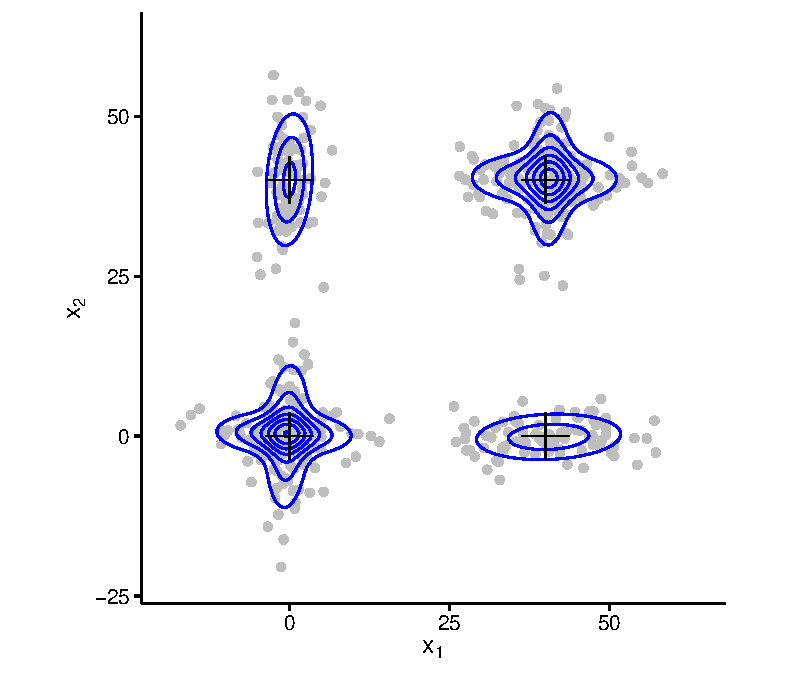
\includegraphics[width=0.7\textwidth]{figures/partition-example-mixture.pdf} \\
 \end{tabular}
 \caption{Density of Gaussian mixture of 6 components. Sample mean estimated of each component is represented by '+'.}\label{ex_mixture}
\end{center}
\end{figure}

Equation~\ref{cluster_criteria} with partition $\mathcal{P}_6 = \{ \{1\},\{2\}, \{3\}, \{4\}, \{5\}, \{6\} \}$ yields to a 6 clusters were each component is associated to one cluster as shown in Figure~\ref{ex_one_one}.

\begin{figure}[h]
\begin{center}
\begin{tabular}{cc}
 %   6 toy mixture
  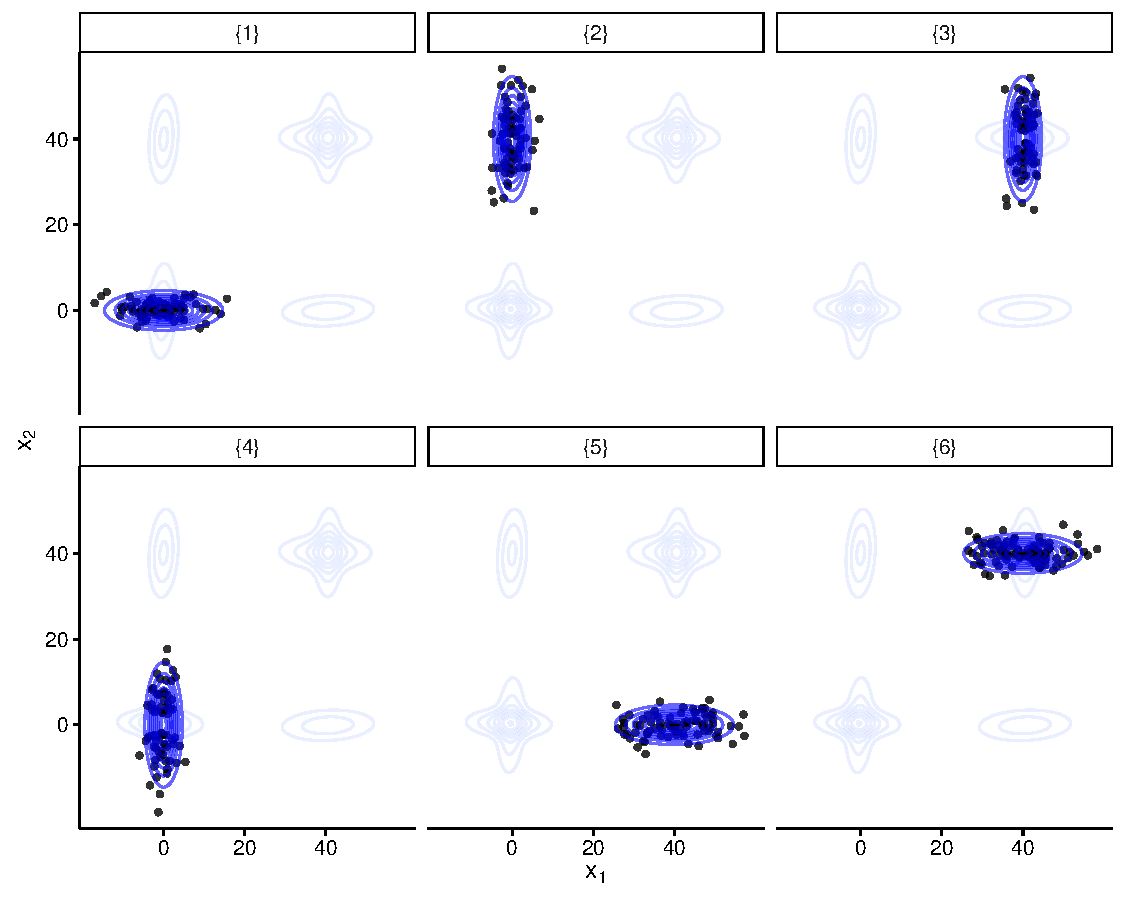
\includegraphics[width=\textwidth]{figures/partition-example-part6.pdf} \\
 \end{tabular}
 \caption{One cluster corresponds to one component}\label{ex_one_one}
\end{center}
\end{figure}

In the partition $\mathcal{P}_4 = \{ \{1, 4\},\{2\}, \{5\}, \{3, 6\} \}$, the componentts 1 and 4 define a single cluster, as well as components 3 and 6. Figure~\ref{ex_two_one} shows the clustering with the iso-density curves defined by each component. In this case, clusters labeled $\{1,4\}$ and $\{3, 6\}$ are modelled by a mixture of two components. The \fmm with partition $\mathcal{P}_4$ is
\begin{itemize}
\item $f_{\{1,4\}} = \frac{1}{2} \phi(\;\cdot\; ;  \m\mu_1, \m\Sigma_1) + \frac{1}{2} \phi(\;\cdot\; ;  \m\mu_4, \m\Sigma_4)$, 
\item $f_{\{2\}} = \phi(\;\cdot\; ;  \m\mu_2, \m\Sigma_2)$, 
\item $f_{\{5\}} = \phi(\;\cdot\; ;  \m\mu_5, \m\Sigma_5)$ and
\item $f_{\{6,3\}} = \frac{1}{2} \phi(\;\cdot\; ;  \m\mu_6, \m\Sigma_6) + \frac{1}{2} \phi(\;\cdot\; ;  \m\mu_3, \m\Sigma_3)$.
\end{itemize}

Using Equation~\ref{cluster_criteria} each observation $\m x_i$ is classified to one component (Figure~\ref{ex_two_one}).

\begin{figure}[h]
\begin{center}
\begin{tabular}{cc}
 %   6 toy mixture
  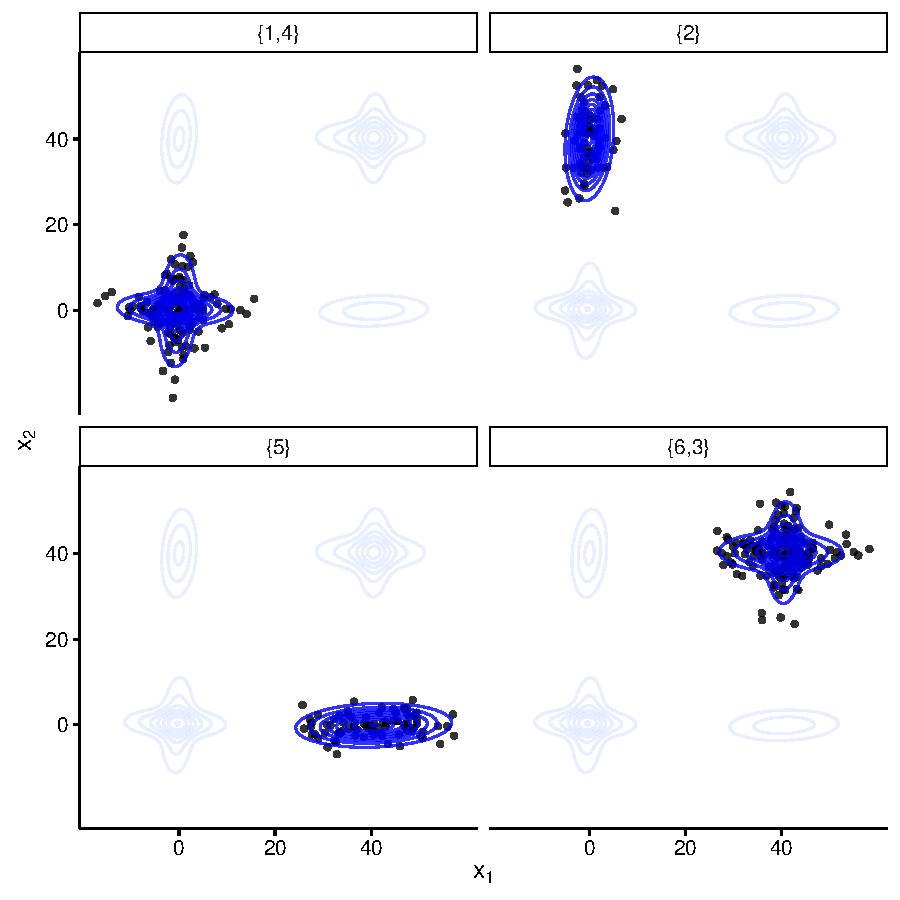
\includegraphics[width=0.65\textwidth]{figures/partition-example-part4.pdf} \\
 \end{tabular}
 \caption{One cluster corresponds to one or more components}\label{ex_two_one}
\end{center}
\end{figure}


The hierarchical sequence of partitions of $\{1, 2, 3, 4, 5, 6\}$ is given by the sequence of partition

\begin{equation}
\begin{array}{r c l}
\mathcal{P}_1 &=& \{\{1, 2, 3, 4, 5, 6\}\}, \\
\mathcal{P}_2 &=& \{\{1, 4, 2, 5\}, \{6, 3\} \},  \\
\mathcal{P}_3 &=& \{\{1, 4, 2\}, \{5\}, \{6, 3\} \}, \\
\mathcal{P}_4 &=& \{\{1, 4\},\{2\}, \{5\}, \{6, 3\} \}, \\
\mathcal{P}_5 &=& \{\{1\},\{2\},\{4\},\{5\},\{6,3\} \},\\
\mathcal{P}_6 &=& \{\{1\},\{2\},\{3\},\{4\},\{5\},\{6\}\}.
\end{array}
\label{hier_ex}
\end{equation}

\section{Building a hierarchical sequence of partitions using posterior probability vectors}\label{generic_merging}

Let $\text{\textbf{X}} = \{\m x_1,\dots,\m x_n \}$ be a sample defined in  a domain $\mathbb{X}$ and let $f$ be a \fmm with $k$ components defined on $\mathbb{X}$ (Equation~\ref{mixt}). Given a partition $\mathcal{P}_s = \{I_1, \dots, I_s\}$, for $i$, $1\leq i \leq n $, let $\m\tau_{i \mathcal{P}_s}= \left( \tau_{i I_1} , \dots, \tau_{i I_s}  \right)$ be the posterior probability vector (Equation~\ref{ppv}) that respectively measures the chances that observation $\m x_i$ was generated by components $f_{I_1}, \dots, f_{I_s}$. In this section we introduce a generic approach to build a hierarchical sequence of partitions using only the information contained on the posterior probability vectors $\{\m\tau_{i \mathcal{P}_s}\}_{1\leq i \leq n}$.


Let $\lambda(\m\tau_{i \mathcal{P}_s},  I_a,  I_b)$ be a function measuring how likely is to merge mixture components $\hat{f}_{I_a}$ and $\hat{f}_{I_b}$ when $\m \tau_{i \mathcal{P}_s}$ is known for any observation $\m x_i$. Let $\omega(\m\tau_{i \mathcal{P}_s},  I_a,  I_b)$ be a function measuring how reliable is the value $\lambda(\m\tau_{i \mathcal{P}_s},  I_a,  I_b)$.  For a given partition $\mathcal{P}_s$ and functions $\lambda$ and $\omega$ we propose to merge those two parts $I_a, I_b \in \mathcal{P}_s$ maximising the weighed mean
\begin{equation}\label{unifying_equation}
S_{\omega, \lambda}( \m\tau_{\mathcal{P}_s},  I_a,  I_b) = \frac{\sum_{i=1}^n \omega(\tau_{i \mathcal{P}_s}, I_a, I_b) \lambda(\tau_{i \mathcal{P}_s}, I_a, I_b)}{\sum_{i=1}^n \omega(\tau_{i \mathcal{P}_s}, I_a, I_b) }.
\end{equation}


Starting from partition $\mathcal{P}_k = \{ \{1\}, \dots, \{k\} \}$ and maximising repeatedly Equation~\ref{unifying_equation} yields to a hierarchical sequence of partitions. The process only depends on the posterior probability vectors and on the definition of functions $\omega$ and $\lambda$. This generic formulation includes a measure of similarity between two components $f_{I_a}$ and $f_{I_b}$ by the definition of function $\lambda$. Functions $\omega$ allows to define weight for the measurement $\lambda$ for an specific observation $\m x_i$.

\section{Functions $\omega$ and $\lambda$}\label{function_examples}

\subsection{Minimising the final entropy}
\label{entropy_section}

The Shannon entropy of a posterior probability vector $\m\tau_{i \mathcal{I}_s} = \left( \hat{\tau}_{i I_1} , \dots, \hat{\tau}_{i I_s}  \right)$ is
\[
\text{Ent}( \m\tau_{i \mathcal{P}_s} ) = \sum_{j=1}^s \tau_{i I_j}  \log(\tau_{i I_j} ).
\]


\cite{baudry2010combining} propose an algorithm to build a hierarchical sequence of partitions. Starting from partition $\mathcal{P}_s = \{ I_1, \dots, I_s\}$ the algorithm iteratively merges  the two components that optimize the entropy. Let $\mathcal{P}_s(I_a\cup I_b)$ be the partition obtained after meging components $I_a$ and $I_b$ from $\mathcal{P}_s$. The two components $I_a$ and $I_b$ that Baudry et al.'s algorithm merges are those that minimises the overall entropy, that is the two components $I_a$ and $I_b$ are merged if
\[
\sum_{i=1}^n \text{Ent}( \m\tau_{i \mathcal{P}_s(I_a\cup I_b)} )
\]
is minimum.


\cite{baudry2010combining}  show that to minimise previous expression is equivalent to maximise the difference
\[
\sum_{i=1}^n \text{Ent}( \m\tau_{i \mathcal{P}_s} ) - \text{Ent}( \m\tau_{i \mathcal{P}_s(I_a\cup I_b)} ).
\]
which can be rewritten in terms of $\m\tau_{i \mathcal{I}_s}$ as
\begin{equation}\label{entropy}
\sum_{i=1}^n  (\tau_{iI_a}+\tau_{iI_b}) \log(\tau_{iI_a} + \tau_{iI_b}) - \left\{ \tau_{iI_a} \log(\tau_{iI_a}) + \tau_{iI_b} \log(\tau_{iI_b}) \right\}.
\end{equation}


The last maximisation problem suggests to define function $\lambda$ as
\[
\lambda(\m\tau_{i \mathcal{P}_s},  I_a,  I_b) =  (\tau_{iI_a}+\tau_{iI_b}) \log(\tau_{iI_a} + \tau_{iI_b}) - \left\{ \tau_{iI_a} \log(\tau_{iI_a}) + \tau_{iI_b} \log(\tau_{iI_b}) \right\}.
\]
which calculates the entropy increment provided by each observation. The expression $S_{\omega, \lambda}( \m\tau_{\mathcal{P}_s},  I_a,  I_b) $ equivalent to the approach presented by \cite{baudry2010combining} is obtained when $\omega$ is constant, for example 
\[
\omega(\m\tau_{i \mathcal{P}_s},  I_a,  I_b) = 1.
\]

In this case Equation~\ref{unifying_equation} takes the form
\[
\begin{split}
S_{\omega, \lambda}( \m\tau_{\mathcal{P}_s},  I_a,  I_b) = \frac{1}{n} \sum_{i=1}^n & (\tau_{iI_a}+\tau_{iI_b}) \log(\tau_{iI_a} + \tau_{iI_b}) - \\ 
&\quad \left\{ \tau_{iI_a} \log(\tau_{iI_a}) + \tau_{iI_b} \log(\tau_{iI_b}) \right\}
\end{split}
\]


\subsection{Maximising the misclassification probability}
\label{missclassification_section}

A different approach is introduced by \cite{hennig2010methods}. He proposes to combine the components $I_a$ and $I_b$ from $ \mathcal{P}_s$ that \emph{the probability of classifying to component $\hat{f}_{I_b}$ an observation generated from component $\hat{f}_{I_a}$ } is maximum.

To estimate this probability,  \cite{hennig2010methods} uses a consistent estimator, the Directed Estimated Misclassification Probabilities (DEMP). The estimate is
\[
\frac{ \frac{1}{n} \sum_{i=1}^n {\tau_{iI_a} \mathbbm{1}\left( \forall j\; \tau_{i I_{b}} \geq \tau_{iI_j} \right)}}{ \hat{\pi}_{I_a}},
\]
where $\mathbbm{1}\left( \cdot \right)$ is the indicator function. Because $ \hat{\pi}_{I_a} = \frac{1}{n} \sum_{i=1}^n \tau_{iI_a}$, the previous estimate can be written in terms of the posterior probability vector as
\begin{equation}\label{demp_criteria}
\frac{ \sum_{i=1}^n {\tau_{iI_a} \mathbbm{1}\left( \forall j\; \tau_{i I_{b}} \geq \tau_{iI_j} \right)}}{\sum_{i=1}^n \tau_{iI_a} }.
\end{equation}

This approach suggests to define
\begin{equation}\label{lambda_demp}
\lambda(\m\tau_{i \mathcal{P}_s},  I_a,  I_b) = \mathbbm{1}\left( \forall j\; \tau_{i I_{b}} \geq \tau_{iI_j} \right)
\end{equation}
and
\[
\omega(\m\tau_{i \mathcal{P}_s},  I_a,  I_b) =  \tau_{iI_a}.
\]

A variation of \cite{hennig2010methods} approach is proposed by \cite{longford2014}. Instead of considering function $\lambda$ given by Equation~\ref{lambda_demp} they propose the of confusion between $f_{I_b}$ and $f_{I_a}$ with function $\lambda$ given by
\[
\lambda(\m\tau_{i \mathcal{P}_s},  I_a,  I_b) = \frac{\tau_{iI_b}}{\tau_{iI_a} + \tau_{iI_b}},
\]
giving another example of function $S_{\omega, \lambda}( \m\tau_{\mathcal{P}_s},  I_a,  I_b)$.


\subsection{Example of function $\omega$}

The motivation behind function $\omega(\m\tau_{i \mathcal{P}_s},  I_a,  I_b) = \tau_{iI_a}$ in (Hennig (2010) and Langford (2014)) is to give more weight to those observations more related to partition $I_a$. A more extremal weighting can be introduced considering only those observation having maximum $ \tau_{iI_a}$, that is
\[
\omega(\m\tau_{i \mathcal{P}_s},  I_a,  I_b) = \mathbbm{1}\left( \forall j\; \tau_{i I_{a}} \geq \tau_{iI_j} \right).
\]

Using the (Longford and..) definition of function $\lambda$, $\lambda(\m\tau_{i \mathcal{P}_s},  I_a,  I_b) = \tau_{iI_b} (\tau_{iI_a} + \tau_{iI_b})^{-1}$, we can define another very simple function measuring how likely is to classify observation into $I_b$ as
\[
\lambda(\m\tau_{i \mathcal{P}_s},  I_a,  I_b) = \tau_{iI_b}.
\]

\section{The logratio approach}\label{logratio_section}

The generic expression of $S_{\omega, \lambda}( \m\tau_{\mathcal{P}_s},  I_a,  I_b)$ (\ref{unifying_equation}) permits to extend the criteria for merging components to expressions defined by the analyst. \cite{aitchison1986statistical} introduces a serie of tools to study samples defined in the Simplex space $\mathcal{S}^d$, i.e $\mathcal{S}^d = \{ (x_1,\dots, x_d) \;|\; x_i > 0 \text{ and } \sum_{i=1}^k x_i = 1 \}$. 

In this section we are interested in different approaches to measure the chances of merging two parts $I_a$ and $I_b$ taking into an account that the posterior probability vector are observations in the Simplex space. In other words we are interested in defining functions $\lambda$ which takes into an account the geometric structure of $\mathcal{S}^d$. We are going to define two new measures, the first ones is motivated by the Entropy notion introduced in \ref{entropy_section}, the second is based on the misclassification definition given in Section~\ref{missclassification_section}.


In \cite{baudry2010combining} confusion between components is measured using the notion that the closer the posterior probability vector is from $(\frac{1}{s}, \dots, \frac{1}{s})$ the more confused are the components (higher is the Entropy).Therefore, to measure the chances of confusing $I_b$ with $I_a$ we can measure how different is $(\frac{\tau_{i I_a}}{\tau_{i I_a} +\tau_{i I_b}}, \frac{\tau_{i I_b}}{\tau_{i I_a} + \tau_{i I_b}})$ from $(\frac{1}{2}, \frac{1}{2})$. That is, we restrict only on the probabilities associated to the components to be merged. To measure this difference we use the squared norm defined in the Simplex space. The squared norm of a posterior probability vector, $\| (\tau_{iI_a}, \tau_{iI_b}) \|^2$  defined by \cite{aitchison2002simplicial} is 
\[
\lambda(\m\tau_{i \mathcal{P}_s},  I_a,  I_b) = \left\| (\tau_{iI_a}, \tau_{iI_b}) \right\|^2 = -\log^2 \left(\frac{ \tau_{iI_b} }{ \tau_{iI_a} }\right).
\]

In \cite{hennig2010methods} the notion of confusion between two components $I_a$ and $I_b$ is measured  using the value $\mathbbm{1}\left( \forall j\; \tau_{i I_{b}} \geq \tau_{i I_j} \right)$. Conditioning that the observation is generated by $I_a$ we propose to measure how likely is to classify an observation to $I_b$ by measuring the relative difference between $\tau_{i I_b}$ and $\tau_{i I_a}$, that is 
\[
\lambda(\m\tau_{i \mathcal{P}_s},  I_a,  I_b) = \log \left(\frac{ \tau_{iI_b} }{ \tau_{iI_a} }\right).
\]

Due the two different methods use logratios they take into an account the geometric properties of the Simplex space \citep{aitchison2002simplicial}.  Moreover, doing so, we can guarantee \emph{subcompositional coherence} in this measurement \citep{aitchison1986statistical}. Another interesting feature when logratio approach is used is the \emph{scale invariance} property, that is, the approach is not restricted to posterior probability vectors but to any other kind of vector giving relative information between each mixture component. Therefore, the methods considered here are suitable to be applied in more general scenarios such that those were instead of posterior probability vectors different weights are given to each part (e.g. weights in fuzzy clustering).

The selection of $\omega(\m\tau_{i \mathcal{P}_s},  I_a,  I_b)$ is of special importance in the logratio approach. When we are considering to merge two components $I_a$ and $I_b$, the ratio for observations that are not representative of this two components (observations far from been classidied into $I_a$ or $I_b$) should be unweight. The main reason is that this posterior probabilitites are subject to a high amount of variability due the small posterior probabilities $\tau_{iI_a}$ and $\tau_{iI_b}$.

Noting that when $\omega(\m\tau_{i \mathcal{P}_s},  I_a,  I_b) =  \tau_{iI_a}$ and $\lambda(\m\tau_{i \mathcal{P}_s},  I_a,  I_b) = \log \left(\frac{ \tau_{iI_b} }{ \tau_{iI_a} }\right)$ are considered, Equation~\ref{unifying_equation} results in
\[
S_{\omega, \lambda}( \m\tau_{\mathcal{P}_s},  I_a,  I_b) = \frac{\sum_{i=1}^n\tau_{iI_a}  \log \left(\frac{ \tau_{iI_b} }{ \tau_{iI_a} }\right)}{\sum_{i=1}^n \tau_{iI_a}}.
\]
For a fixed component $I_a$, the expression can be interpreted as the Kullback-Leibler divergence (in negative sign) comparing the distribution of classifiying observations $x_i \in X$ to $I_a$ against the distributions of classifying the same observations to $I_b$. The approach merges those two component with the lower Kullback-Leibler divergence.

\section{Merging components in a finite mixture: examples}\label{merging_examples_dist}

\subsection{Merging components in a mixture of Gaussian distributions}

In Section~\ref{example} we generated a sample of 500 observations coming from a mixture with 6 components. 


Considering $\omega = 1$ and $\lambda = (\tau_{iI_a}+\tau_{iI_b}) \log(\tau_{iI_a} + \tau_{iI_b}) - \left\{ \tau_{iI_a} \log(\tau_{iI_a}) + \tau_{iI_b} \log(\tau_{iI_b}) \right\}$ that is themethod proposed by \cite{baudry2010combining} we obtained the sequential hierarchical partition given by Equation~\ref{hier_ex}. When we consider  the DEMP approach introduced in \citep{hennig2010methods}, i.e. $\omega = \tau_{i I_a}$ and $\lambda = \mathbbm{1}\left( \forall j\; \tau_{i I_{b}} \geq \tau_{iI_j} \right)$ the sequential hierarchical obtained is
\begin{equation}
\begin{array}{r c l}
\mathcal{P}_1 &=& \{\{1, 2, 3, 4, 5, 6\}\}, \\
\mathcal{P}_2 &=& \{\{1, 4, 2, 5\}, \{6, 3\} \},  \\
\mathcal{P}_3 &=& \{\{1, 4, 2\}, \{5\}, \{6, 3\} \}, \\
\mathcal{P}_4 &=& \{\{1, 4\},\{2\}, \{5\}, \{6, 3\} \}, \\
\mathcal{P}_5 &=& \{\{1, 4\},\{2\}, \{3\},\{5\},\{6\} \},\\
\mathcal{P}_6 &=& \{\{1\},\{2\},\{3\},\{4\},\{5\},\{6\}\}.
\end{array}
\end{equation}

This sequence only differs from the Baudry's in the partition $\mathcal{P}_5$.  Figure~\ref{gaussian_Svalues} shows the value of function $S$ given by Equation~\ref{unifying_equation}. In these values the largest change is detected in the step from 4 clusters to consider 3 clusters. This reduction suggests that the correct number of clusters is given by 4 clusters.
\begin{figure}[t]
\begin{center}
\begin{tabular}{cc}
  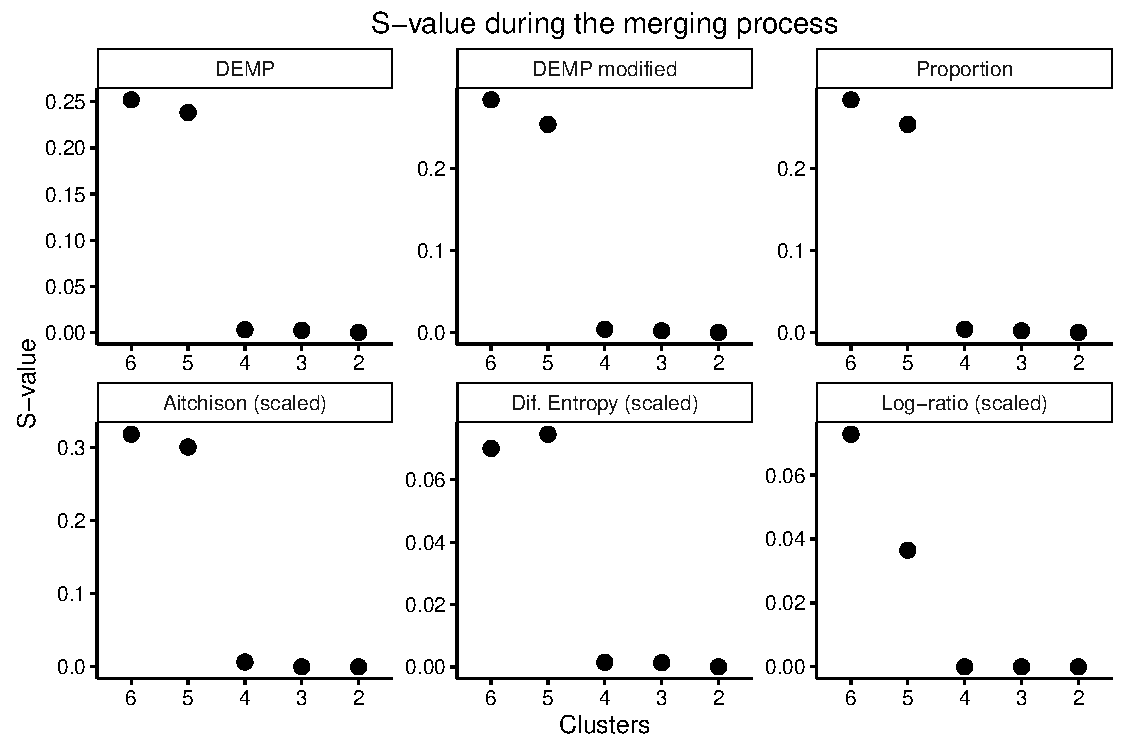
\includegraphics[width=0.85\textwidth]{figures/gaussian_Svalues.pdf} \\
 \end{tabular}
 \caption{S-values obtained using the approaches presented by Baudry et al. and Hennig labeled Entropy and DEMP respectively.}\label{gaussian_Svalues}
\end{center}
\end{figure}

\subsection{Merging components in a mixture of multinomial distributions}

Merging approaches presented in this article rely on the vector of posterior probabilities this can be calculated for any finite mixture model. In this section we present the case of a finite mixture of multinomial distribution.

Pigs dataset can be obtained from package \pkg{zCompositions} R package \citep{palarea2012zcompositions}. The dataset contains data of 29 sows. In different moments the pigs were recorder during 5 minutes and its current activity was registered. For each pig six locations were considered: straw bed (BED), half in the straw bed (HALF.BED), dunging passage (PASSAGE), half in the dunging passage (HALF.PASS), feeder (FEEDER) and half in the feeder (HALF.FEED). Although the original dataset has 6 different activities, to avoid identifiability problems (Teicher, 1960; Blischke, 1964; Titterington et al., 1985) we eliminate the HALF.PASS, HALF.FEED, HALF.BED which have a very small number of events.

We have used \pkg{mixtools} \citep{benaglia2009mixtools} to fit the mulitinomial mixture. 9 components were identified as optimum according to BIC criterion. In Figure~\ref{multinomial_mixture} the bar plot for each component. That is considering Equation~\ref{map_criteria} or Equation~\ref{cluster_criteria} with partition $\mathcal{P}_9 = \{\{1\}, \{2\}, \{3\}, \{4\}, \{5\}, \{6\}, \{7\}, \{8\}, \{9\} \}$.

\begin{figure}[t]
\begin{center}
\begin{tabular}{cc}
  \includegraphics[width=0.95\textwidth]{figures/multinomial_mixt.pdf} \\
 \end{tabular}
 \caption{Components after adjusting a 9 mixture of multinomial distributions}\label{multinomial_mixture}
\end{center}
\end{figure}

Considering $\omega = \tau_{i I_a}$ and $\lambda = -\log^2 \left(\frac{ \tau_{iI_b} }{ \tau_{iI_a} }\right)$ we obtained the sequential hierarchical partition given by


\begin{equation}
\begin{array}{r c l}
\mathcal{P}_1 &=& \{\{1,2,3,4,5,6\}\}, \\ 
\mathcal{P}_2 &=& \{\{1,2,4\},\{3,5,6\}\}, \\ 
\mathcal{P}_3 &=& \{\{1,2,4\},\{3,5\},\{6\}\}, \\ 
\mathcal{P}_4 &=& \{\{1,4\},\{2\},\{3,5\},\{6\}\}, \\ 
\mathcal{P}_5 &=& \{\{1\},\{2\},\{3,5\},\{4\},\{6\}\}, \\ 
\mathcal{P}_6 &=& \{\{1\},\{2\},\{3\},\{4\},\{5\},\{6\} \}.
\end{array}
\label{hier_ex_multinomial}
\end{equation}

Figure~\ref{multinomial_Svalues} shows the $S$-value's (Equation~\ref{unifying_equation}) obtained in each step. During step 5, 4 and 3 the score is close to 0 (-62, -74, -80 respectively). When merging from 3 to 2 component the score is reduced notably (-7966). This reduction suggests that when merging from 3 to 2 clusters we are losing valuable information, and therefore, it seems reasonable to stop at 3 clusters.

\begin{figure}[t]
\begin{center}
\begin{tabular}{cc}
  \includegraphics[width=0.65\textwidth]{figures/multinomial_Svalues.pdf} \\
 \end{tabular}
 \caption{S-values obtained using the Aitchison $\lambda = -\log^2 \left(\frac{ \tau_{iI_b} }{ \tau_{iI_a} }\right)$ and $\omega = \tau_{i I_a}$ in the multinomial example.}\label{multinomial_Svalues}
\end{center}
\end{figure}

Figure~\ref{multinomial_clust3} show the final 3 clusters. The first cluster contains components 1, 2 and 4, all of them represented by sows with a high amount of time feeding. The scond cluster contains components 3 and 5, this cluster is characterized by with sows with high ammount of time in bed. Finally, the thirs cluster is form with a single component 6 wich have a higher amount of time in the passage.

\begin{figure}[t]
\begin{center}
\begin{tabular}{cc}
  \includegraphics[width=0.95\textwidth]{figures/multinomial_clust3.pdf} \\
 \end{tabular}
 \caption{Components after clustering the 9 mixture components in a 3-\fmm}\label{multinomial_clust3}
\end{center}
\end{figure}

\section{Discussion}

When \fmm is used in clustering the question \textit{``is a cluster determined by a unique component?''} emerges. Different authors have proposed scenarios where it seems reasonable to argue that a cluster can be better model by more than one single component, or equivalently, modelled by a \fmm itself. In this scenarios, the approaches proposed in this article can be of interest.

In literature different approaches have been considered to merge the components of a finite mixture. Some of them are specific to a particular type of mixture (methods related to gaussian mixtures) and some others are independent of the type of mixture (to cite generic approaches). The generic approach proposed in this articles only relies  on the posterior probability vectors therefore it is independent from the family of mixture and can be applied with any \fmm.

We would like to notice that the approach presented in this article uses the posterior probability vectors which come from a finite mixture model. Some methods presented Because the methods only use information, it make sense to apply the methods presented here in other scenarios were a vector of posterior probabilities is given in advance.

Not less important is to mention how simple it becomes to evaluate the $S$-values when function $\omega(\m\tau_{i \mathcal{P}_s},  I_a,  I_b) = \tau_{iI_a}$ and $\lambda(\m\tau_{i \mathcal{P}_s},  I_a,  I_b) = \tau_{iI_b}$ are considered. Also, we would like to highlight the guaranteed properties obtained if the logratio approaches are considered as introduced in Section~\ref{logratio_section}.

Finally, in the examples shown in this article we have used descriptives criteria to stop the merging process by controlling the $S$-values. We notice here that different definitions of functions $\lambda$ and $\omega$ rises different way to interpret the $S$-values, therefore, it is mandatory to take into an account the interpretation of $S$-values before defining an stopping criteria.


%%% BIBLIOGRAPHY
\newpage

\bibliographystyle{apalike}
\begin{thebibliography}{}

\bibitem[Aitchison, 1986]{aitchison1986statistical}
Aitchison, J. (1986).
\newblock {\em {The Statistical Analysis of Compositional Data}}.
\newblock Monographs on Statistics and Applied Probability. Chapman \& Hall
  Ltd., London (UK).

\bibitem[Aitchison, 2002]{aitchison2002simplicial}
Aitchison, J. (2002).
\newblock {\em {Simplicial inference}}.
\newblock {\em Algebraic Methods in Statistics anb Probability}, 287: 1--22.

\bibitem[Baudry et~al., 2010]{baudry2010combining}
Baudry, J.P., Raftery, A.~E., Celeux, G., Lo, K., and Gottardo, R. (2010).
\newblock {Combining Mixture Components for Clustering}.

\bibitem[Fraley, 2002]{fraley2002model}
Fraley, C. and Raftery, A. E. (2002).
\newblock {Model-Based Clustering, Discriminant Analysis, and Density Estimation}.
\newblock {\em Journal of the American Statistical Association}, 97(458): 611–631.

\bibitem[Hennig, 2010]{hennig2010methods}
Hennig, C. (2010).
\newblock {Methods for merging Gaussian mixture components}.
\newblock {\em Advances in Data Analysis and Classification}, 4(1):3--34.

\bibitem[Lee and Cho, 2004]{lee2004combining}
Lee, H.J. and Cho, S. (2004).
\newblock {Combining Gaussian Mixture Models}.
\newblock In Yang, Z., Yin, H., and Everson, R., editors, {\em Intelligent Data
  Engineering and Automated Learning – IDEAL 2004 SE - 98}, volume 3177 of
  {\em Lecture Notes in Computer Science}, pages 666--671. Springer Berlin
  Heidelberg.

\bibitem[Longford and Bartosova, 2014]{longford2014}
Longford, N.~T. and Bartosova, J. (2014).
\newblock {A confusion index for measuring separation and clustering}.
\newblock {\em Statistical Modelling}, 14(3):229--255.

%\bibitem[Meila, 2006]{meila2006comparing}
%Meila, M (2006).
%\newblock {Comparing clusterings - an information based distance}.
%\newblock {\em Journal of Multivariate Analysis}, 98:873--895.

\bibitem[Melnykov, 2013]{melnykov2013distribution}
Melnykov, V. (2013).
\newblock {On the Distribution of Posterior Probabilities in Finite Mixture
  Models with Application in Clustering}.
\newblock {\em Journal of Multivariate Analysis}, 122:175--189.

%\bibitem[Melnykov et~al., 2012]{melnikov2012mixsim}
%Melnykov, V. and Chen, W.C. and Maitra, R. (2012).
%\newblock {MixSim: An R Package for Simulating Data to Study Performance of Clustering Algorithms}.
%\newblock {\em Journal of Statistical Software}, 51(12).

\bibitem[Palarea-Albaladejo and Martin-Fernandez (2012)]{palarea2012zcompositions}
Palarea-Albaladejo J. and Martin-Fernandez J.A. (2012).
\newblock {zCompositions: Imputation of Zeros and Nondetects in Compositional Data Sets}.
\newblock {\em R package version 1.0.3}.

\bibitem[Pastore and Tonellato, 2013]{pastore2013merging}
Pastore, A. and Tonellato, S.~F. (2013).
\newblock {A Merging Algorithm for Gaussian Mixture Components}.
\newblock {\em SSRN Electronic Journal}, (04).

\bibitem[Benaglia et~al., 2009]{benaglia2009mixtools}
Benaglia, T., Chauveau, D., Hunter, D.R. and Youn, R. (2009).
\newblock {mixtools: An R Package for Analyzing Finite Mixture Models}.
\newblock {\em Journal of Statistical Software}, 32(6), 1-29.

\end{thebibliography}

%%%%%%%%%%% END SPACING
\end{spacing}

\end{document}
